\documentclass{article}

% Importing document settings from our file "packages.sty"
\usepackage{packages}

\fancyhead{} % clear all header fields
\fancyhead[LO]{\textbf{Vigdis-Irene Steinsund, \\ Thomas Hasvold}}
\fancyhead[CO]{\textbf{TDT4136 - Assignment 3}}
\fancyhead[RO]{\textbf{06/10/2023}}

% Beginning of document
\begin{document}

    % Defining main matter settings (Norsk: innstillinger for hoveddelen av teksten)
    \mainmatter

    \section*{Easy}

    \begin{figure}[H]
        \centering
        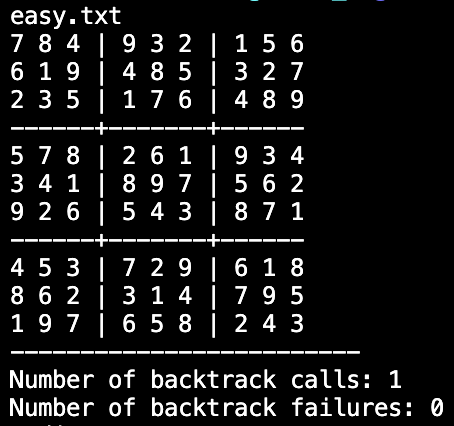
\includegraphics[width=0.5\textwidth]{Images/easy.png}
        \caption[Easy solution]{Solution for the easy sudoku board. The backtrack function was called only once, and there were no instances in which the backtrack function returned a failure.}
        \label{fig:Easy solution}
    \end{figure}

    \section*{Medium}

    \begin{figure}[H]
        \centering
        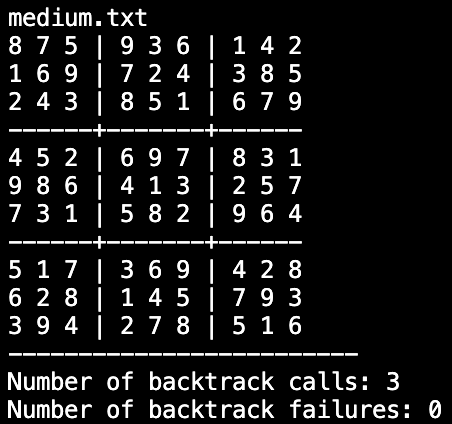
\includegraphics[width=0.5\textwidth]{Images/medium.png}
        \caption[Medium solution]{Solution for the medium sudoku board. The backtrack function was called a total of 3 times, and there were still no instances in which the backtrack function returned a failure.}
        \label{fig:Medium solution}
    \end{figure}

    \section*{Hard}

    \begin{figure}[H]
        \centering
        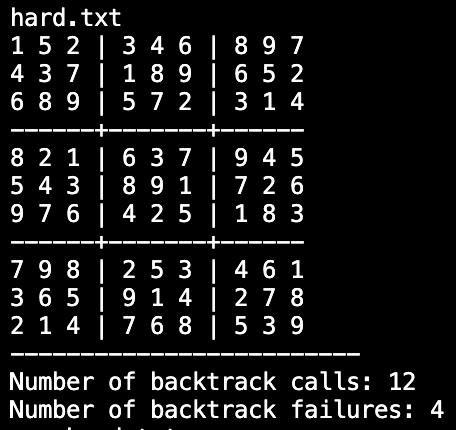
\includegraphics[width=0.5\textwidth]{Images/hard.png}
        \caption[Hard solution]{Solution for the hard sudoku board. The backtrack function was called a total of 12 times, and there were 4 instances in which the function returned a failure.}
        \label{fig:Hard solution}
    \end{figure}

    \section*{Very hard}

    \begin{figure}[H]
        \centering
        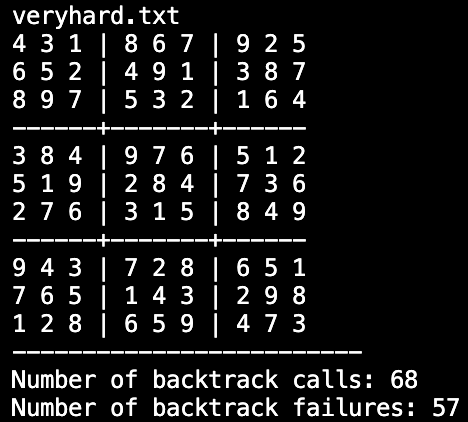
\includegraphics[width=0.5\textwidth]{Images/very_hard.png}
        \caption[Very hard solution]{Solution for the very hard sudoku board. In this solution, the backtrack function was called a total of 68 times, and a total of 57 failures were returned.}
        \label{fig:Very hard solution}
    \end{figure}

    We see in the results that the backtrack function was called around 1 - 12 
    times in total for the first three boards, and the first four times failures
    were returned was in the hard puzzle. The very hard puzzle however, had a total
    of 68 calls to the backtrack function, and 57 of those calls returned a failure.
    This makes sense since the easier puzzles have more filled cells, and thus
    less empty cells to fill, which reduces the search space for the backtracking
    algorithm, and it therefore needs fewer calls to the backtrack function and will also
    not encounter failures as often. On the other hand, the very hard puzzle has a lot
    fewer filled cells, which means the algorithm must explore a higher number of possibilities,
    in addition to these attempts also leading to more invalid states, when it returns 
    a failure. 

% End of document
\end{document}
